\chapter{Alternative Design \#1- Steel Plate Girder}\label{sec:2}

\section{General Description of Design Alternative}\label{sec:2.1}

The use of steel plate girders as the main component of the superstructure is a viable alternative for the 125 foot, single-span bridge in question. While providing a cost-effective alternative, steel plate girders are capable of handling the load requirements for this bridge must meet under the given conditions. In this case, the girders would bear onto the concrete abutments through the use of elastomeric bearings for each beam. Lateral bracing would be included in the final superstructure design as necessary.

\section{Assumptions Made}\label{sec:2.2}


\begin{figure}[H]
\centering
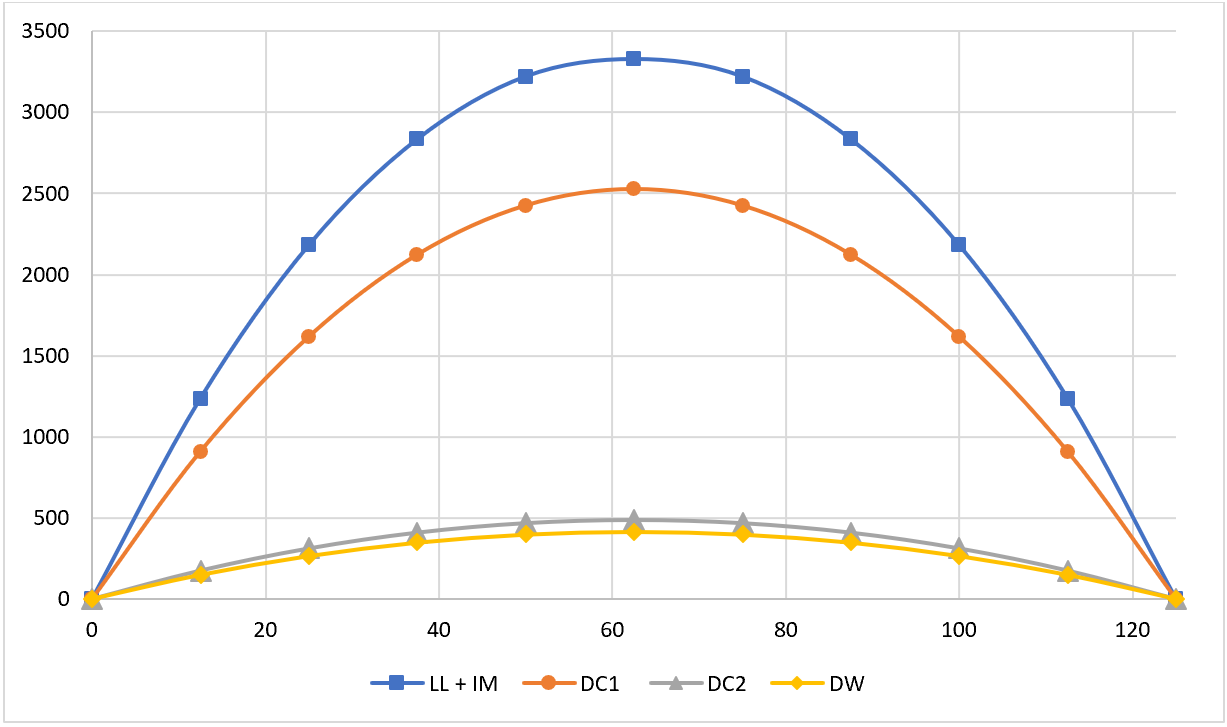
\includegraphics[width=0.75\textwidth]{./appendix/figures/DeadLiveMoment.PNG}
\caption[Alternative Design \#1- Steel Plate Girder: Dead \& Live Load Moments]
{Dead \& Live Load Moments (ft-kip)}\label{fig:dlmome}
\end{figure}

\begin{figure}[H]
	\centering
	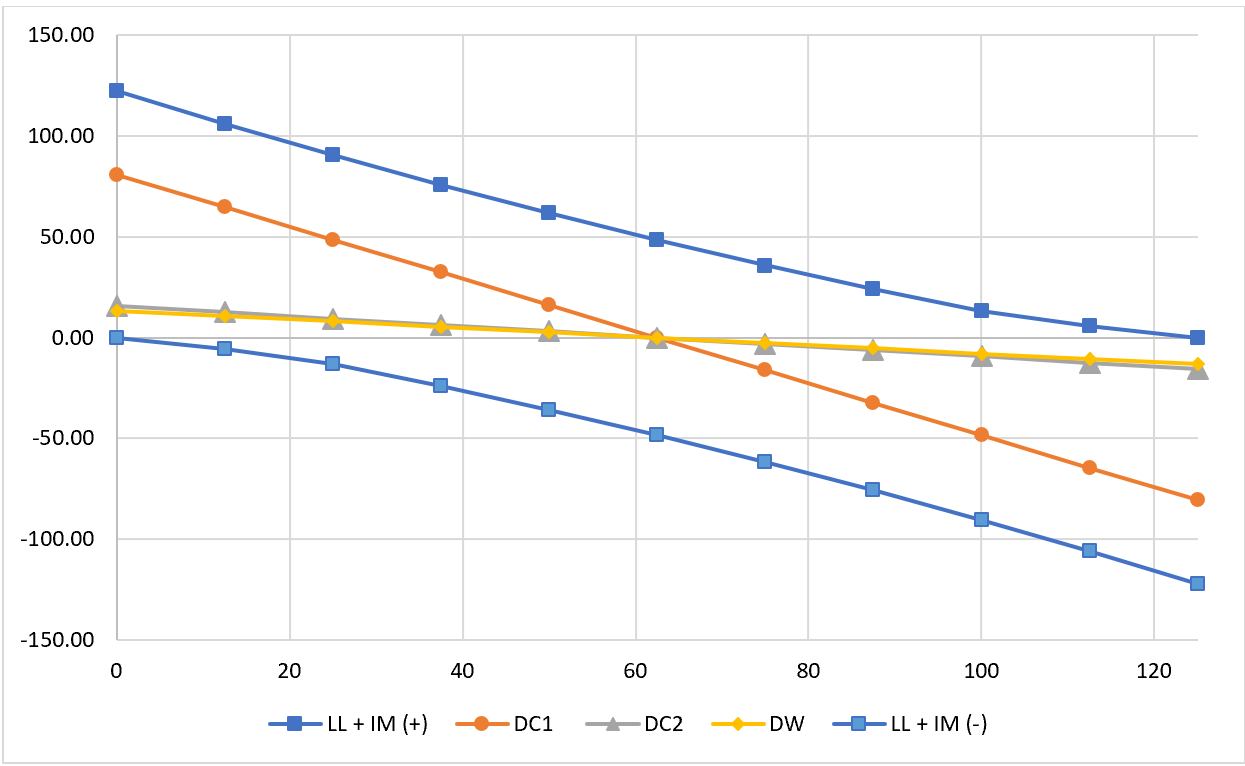
\includegraphics[width=0.75\textwidth]{./appendix/figures/DeadLiveShear.PNG}
	\caption[Alternative Design \#1- Steel Plate Girder: Dead \& Live Load Shears]
	{Dead \& Live Load Shear (kip)}\label{fig:dlshear}
\end{figure}

From Figures~\ref{fig:dlmome} and~\ref{fig:dlshear} it can be seen that 100 feet along the length of the span there exists a desirable balance where the magnitudes of the shear and moments generated are relatively minimized. Therefore, it was determined that the splice would be located at this point. In keeping with this decision, the design of the steel plate girder calls for two sections, fabricated to be 100 feet and 25 feet respectively, spliced together at the previously determined location.

\section{Design Details}
Each steel plate girder consists of three plates, the top flange plate, the web plate, and the bottom flange plate, welded together.

According to AASHTO Table 6.4.1-1 ``Minimum Mechanical Properties of Structural Steel by Shape, Strength, and Thickness,''~\cite{aashto7} the plates will be constructed of AASHTO M 270 (ASTM 709M) Grade 50 Steel, which provides a minimum yield strength, denoted \(F_{y}\), of 50 ksi and a minimum tensile strength, denoted \(F_{u}\), of 65 ksi. Table~\ref{tab:pgdim} displays each girder components' calculated dimensions. These calculations, along with a number of other preliminary calculations, can be found in Appendix~\ref{misc:prelimcalc}.

\begin{table}[H]
\begin{center}
\caption{Plate Girder Components Dimensions}\label{tab:pgdim}
\vspace{0.5cm}
\scalebox{1.0}{
\begin{tabular}{lcc}
\toprule
\midrule
\textbf{Component}              & \textbf{Thickness (in)}  & \textbf{Width (in)} \\
\midrule
\emph{Top Flange}               & 0.75                     & 16.00   \\
\emph{Web}                      & 55                       & 0.5     \\
\emph{Bottom Flange}            & 1.25                     & 16.00   \\
\bottomrule
\end{tabular}}
\end{center}
\end{table}

For Alternative \#1, the cross section of the bridge consists of 4 plate girders, spaced 9.0 feet apart, measured center-to-center. The cross sectional geometry described here can be viewed in Appendix~\ref{cad:spcross}. The beams will be seated on 18 inch x 20 inch x 5.875 inch elastomeric bearing pads with steel plate reinforcement. The source of the dimensions of the elastomeric bearing pads can be found in Appendix~\ref{misc:espan}.  A total of 8 elastomeric bearings will be utilized in this design. As discussed in Section~\ref{sec:2.2}, the plate girders will be spliced together at the 100 foot mark, to accommodate the provided shipping limits, using AASHTO M 164 Type 3 Bolts, which are \(\frac{7}{8}\) inch diameter, and steel plates of varying size. A total of 328 bolts will be utilized for the connection on each beam, totaling 1312 bolts for all four girders. Table~\ref{tab:spdim} details the steel plates utilized in the spliced connection.


\begin{table}[H]
\centering
\caption{Splice Plate Dimensions}\label{tab:spdim}
\vspace{0.5cm}
\scalebox{0.9}{
\begin{tabular}{lrrr}
\toprule
\midrule
\textbf{Component}   & \textbf{Plate Thickness (in)} & \textbf{Plate Dimensions (in\(\times\)in)}    & \textbf{Number of Plates}              \\\midrule
\emph{Top Flange}    & \makecell{0.5\\0.5}           & \makecell{16\(\times\)39.5\\7.5\(\times\)39.5}       & \makecell[r]{1 (top)\\2(bottom)} \\\midrule
\emph{Web}           & 0.5                           & 45\(\times\)34                                       & 2                                 \\ \midrule
\emph{Bottom Flange} & \makecell{1.0\\1.0}           & \makecell{69.5\(\times\)8.5 \\69.5\(\times\)16 }     & \makecell[r]{2 (top)\\1(bottom)}   \\ \bottomrule
\end{tabular}}
\end{table}


This cross-sectional geometry provides for a deck overhang of 2 feet 10 inches, which satisfies the minimum overhang of 27 inches required by Section 3.2.1.1 of~\cite{bridgedesignman}. The deck will be a total of  9 inches in thickness, with 1 inch being for wearing surface. The deck will contain two layers of \#5 reinforcement, one layer will run parallel to the skew of the bridge and the other will run perpendicular to traffic. The layer of reinforcement running parallel to traffic will contain 22 \#5 bars and be spaced at 18 inches. The layer of reinforcement running perpendicular to traffic will contain 83 \#5 bars spaced at 18 inches. The deck surface will contain 2 TL-3 Type F (32 inch) barrier, according to Section 3.2.2 of~\cite{bridgedesignman}.


\section{Quantity Estimates}
The quantities detailed in the following tables were estimated for the plate girder design, using both raw material weights and linear footage quantities.

Table~\ref{tab:spgquant} displays the quantities for the plate girder steel. Table~\ref{tab:babquant} displays the quantities for the bearings and bolts. Table~\ref{tab:concquant} displays the concrete quantities incorporated into this design.

\begin{table}[H]
\centering
\caption{Steel Plate Girder Quantities}\label{tab:spgquant}
\vspace{0.5cm}
\scalebox{0.75}{
\begin{tabular}{lrrrrrrrr}
\toprule
\midrule
\textbf{Part}   & \textbf{\makecell{Length\\ (ft)}}  & \textbf{\makecell{Width\\(ft)}} & \textbf{\makecell{Thickness\\(ft)}} &\textbf{\makecell{Volume\\(ft$^{3}$)}} & \textbf{\makecell{Number\\Required}} & \textbf{\makecell{Weight per\\Part}} & \textbf{\makecell{Total Weight\\(lbs)}} & \textbf{\makecell{LF of Steel\\Girders}} \\
\midrule
\emph{Top Flange}    & 125 & 1.333 & 0.063 & 10.417 & 4 & 20417     & 20417  & 500 \\
\emph{Web}           & 125 & 4.583 & 0.042 & 23.872 & 4 & 11697.049 & 46788  & 500  \\
\emph{Bottom Flange} & 125 & 1.33  & 0.104 & 17.361 & 4 & 5104.167  & 34028  & 500   \\ \midrule
Total   &     &       &       &        &   &           & 101233 & 1500                \\ \bottomrule
\end{tabular}}
\end{table}

\begin{table}[H]
\centering
\caption{Bearing and Bolt Quantities}~\label{tab:babquant}
\scalebox{0.75}{
\begin{tabular}{lccccc}
\toprule\midrule
\textbf{Part}                   & \textbf{Length (in)}  & \textbf{Width (in)} & \textbf{Thickness (in)} & \textbf{\makecell{Number Required\\ per Beam}} & \textbf{\makecell{Total Number\\ Required}} \\ \midrule
\emph{Elastomeric Bearing Pads} & 20                    & 18                  & 5.875                   & 2                                              & 8                                            \\
\emph{AASHTO M 164 Bolts}       &                       &                     &                         & 328                                            & 1312                                          \\ \bottomrule
\end{tabular}}
\end{table}


\begin{table}[H]
\centering
\caption{Concrete Quantities}\label{tab:concquant}
\scalebox{0.65}{
\begin{tabular}{p{4.5cm} r r r r r r r r}
\toprule\midrule
\textbf{Part}   & \textbf{\makecell{Length\\ (ft)}}  & \textbf{\makecell{Width\\(ft)}} & \textbf{\makecell{Thickness\\(ft)}} &\textbf{\makecell{Volume\\(ft\(^{3}\))}} & \textbf{\makecell{Number\\Required}} & \textbf{\makecell{Weight per\\Part}} & \textbf{\makecell{Total Weight\\(lbs)}} & \textbf{\makecell{LF of Steel\\Girders}} \\ \midrule
\emph{Concrete Deck}                                                       & 125 & 1.333   & 0.063 & 10.417   & 4 & 20417       & 20417       & 500    \\ \midrule
\emph{Type V Median Parapet Class B Concrete (assuming rectangular shape)} & 125 & 0.79167 & 2.667 & 263.9219 & 2 & 38268.67188 & 76537.34375 & 250     \\ \midrule
Total:                                                                     &     &         &       &          &   &             & 484350      & 375      \\ \bottomrule
\end{tabular}}
\end{table}


\section{Scheduling Estimates}
According to information provided in Appendix~\ref{misc:costest}, it is estimated that the Steel Plate Girder Alternative would take approximately 6 work weeks to complete. This estimate does not include any delays related to manufacturing, shipping, or construction issues due to weather and it assumes 40 hour work weeks. We felt this assumption was justified by using this assumption uniformly for each alternative.  At this stage our goal is simply to find reasonable approximations for our chosen alternatives to facilitate and inform the selection process.


\section{Cost Estimates}\label{sec:2.6}
The cost analysis for the Steel Plate Girder Alternative excludes any project features that all three alternatives shared. In other words, the cost analysis only considered costs that were specific to the Steel Plate Girder and were the result of characteristics unique to the alternative. Features excluded contain but are not limited, to the concrete deck, deck formwork, parapet walls, and labor for these features.

Due to uncertainties inherent to the the preliminary alternatives phase, assumptions were made to try to get a more accurate estimate. A quote for the Steel Plate Girders were given from West Virginia Steel Cooperation on 2/28/2019 for the amount of \$42,000 per 125 foot girder. The quote is attached in Appendix~\ref{misc:costest}. This quote was deemed valid despite our 100 ft shipping limitation due to the fact that the overall amount of steel will be essentially the same.  This assumption could very well be conservative due to the fact that 125 foot girders are something of a specialty commodity while 100 ft girders are likely more common and 25 ft girders are certainly more common. As a result there exists a potential to benefit from purchasing more standard sized girders than our single 125 foot girder.

 An online crane calculator was used to determine the minimum sized crane necessary to lift the girder into place using the weight of the load and the radius that the crane has to carry the load outward as parameters. It was determined that the minimum crane size required to place the steel plate girders is a 100 ton crane. Due to a lack of reliable contacts, the shipping was estimated to be 10\% of the girders cost. This rate is used in each alternative's cost estimate, however the actual cost of shipping will vary for each alternative.

 A 5\% lump sum was added to account for sheer studs and any other miscellaneous features that might have not been taken into consideration. Markups were assumed and added to the total project cost. These include a running percent of 15\% on job office overhead (Primary Contractor), 15\% on home office overhead (Primary Contractor), 10\% on Profit (Primary Contractor), 2\% on bond (Primary Contractor), and 6\% on taxes (Project). Sub-contractors also have a 25\% running percent that includes job office overhead and profit. The direct cost of this alternative came out to roughly \$295,000 with a project cost of \$445,000. Of the three alternatives analyzed the Steel Plate Girders were founded to be the most economically feasible. A more detailed breakdown can be found in Appendix~\ref{misc:costest}.

\begin{table}[H]
\centering
\caption{Steel Plate Girder Alternative Cost}
\vspace{0.5cm}
\scalebox{0.85}{
\begin{tabular}{p{4cm}rrrrr}\toprule\midrule
\textbf{Description}                                     & \textbf{Quantity} & \textbf{UOM}  & \textbf{Contractor} & \textbf{Direct Cost} &\textbf{Project Cost} \\   \midrule
Steel Plate Girders: Grade 50, 125 feet long                                                                                     & 4      & EA & Prime & \$178,080 & \$264,243 \\ \midrule
Steel Plate Girder Installation                                                                                                  & 80     & HR & Prime & \$69,291  & \$102,817  \\ \midrule
Shipping for Steel Plate Girder                                                                                                  & 1      & LS & Sub   & \$19,130  & \$35,483    \\ \midrule
Splice Connection Installation: Crane-40 Ton                                                                                     & 4      & EA & Prime & \$3168    & \$4701       \\ \midrule
Steel Plate Girder Misc: (Bolts, Sheer Studs, etc)                                                                               & 1      & LS & Prime & \$9,540   & \$14,156      \\ \midrule
M 164 Type 3 Bolts, $\frac{7}{8}$ inch diameter, includes nut \& washer                                                          & 1312   & EA & Prime & \$8193    & \$12,157       \\ \midrule
Top Flange: Steel Plate, structural, for connections \&  stiffeners, $\frac{1}{2}$ inch T, shop fabricated, includes shop primer & 4898   & SI & Prime & \$973     & \$1,444         \\ \midrule
Bottom Flange: Steel Plate, structural, for connections \&  stiffeners, 1 inch T, shop fabricated, includes shop primer          & 9174   & SI & Prime & \$1768    & \$2623           \\ \midrule
Top Flange: Steel Plate, structural, for connections \& stiffeners, $\frac{1}{2}$ inch T, shop fabricated, includes shop primer  & 12,240 & SI & Prime & \$2432    & \$3609            \\ \midrule
Total & & & &  \$295,000 & \$455,000  \\\bottomrule
\end{tabular}}
\end{table}

\section{Sustainability-Related Issues}
During the preliminary design performed for the alternatives phase, there were no sustainability issues observed with this alternative.